\begin{pastexam}[label={px:nccu-111-dsa-06}]{政大資科所 111 學年度 第 6 題}
（追蹤）

(10\%) Use Kruskal's algorithm to find the minimum spanning tree of the graph, $G$, with vertices $\{v_1, v_2, v_3, v_4, v_5, v_6\}$ and the adjust matrix $A$.
\[
A=\begin{pmatrix}
0 & 10 & 16 & 18 & 13 & 8 \\
10 & 0 & 14 & 17 & 15 & 9 \\
16 & 14 & 0 & 9 & 10 & 12 \\
18 & 17 & 9 & 0 & 9 & 19 \\
13 & 15 & 10 & 9 & 0 & 11 \\
8 & 9 & 12 & 19 & 11 & 0
\end{pmatrix}\text{, where } A[i,j] \text{ is the weight of the edge between } v_i \text{ and } v_j
\]
\end{pastexam}

\begin{pastsoln}
答案：最小生成樹的邊是 $(v_1, v_6)$、$(v_2, v_6)$、$(v_3, v_4)$、$(v_4, v_5)$、$(v_5, v_6)$，總權重
$8 + 9 + 9 + 9 + 11 = 46$。

題目的「adjust matrix」是 adjacency matrix（鄰接矩陣）的筆誤。 矩陣對稱，對角線是 $0$，其餘
$15$ 個位置都不是 $0$，所以 $G$ 是 $6$ 個頂點的完全圖，有 $\binom{6}{2} = 15$ 條邊，只看上三角就好。

\textbf{Kruskal}（資結書第~24.2~節、虛擬碼~24.2）：邊依權重由小到大看，兩端已經在同一個集合（加進來
會成環）就跳過，否則加入並合併兩個集合；加滿 $6 - 1 = 5$ 條就停。
\begin{center}
\small
\begin{tabular}{clll}
\toprule
權重 & 邊 & 結果 & 加入後的集合（只列兩個點以上的） \\
\midrule
8 & $(v_1, v_6)$ & 加入（第 1 條） & $\{v_1, v_6\}$ \\
9 & $(v_2, v_6)$ & 加入（第 2 條） & $\{v_1, v_2, v_6\}$ \\
9 & $(v_3, v_4)$ & 加入（第 3 條） & $\{v_1, v_2, v_6\}$, $\{v_3, v_4\}$ \\
9 & $(v_4, v_5)$ & 加入（第 4 條） & $\{v_1, v_2, v_6\}$, $\{v_3, v_4, v_5\}$ \\
10 & $(v_1, v_2)$ & 跳過（同在 $\{v_1, v_2, v_6\}$） & \\
10 & $(v_3, v_5)$ & 跳過（同在 $\{v_3, v_4, v_5\}$） & \\
11 & $(v_5, v_6)$ & 加入（第 5 條） & $\{v_1, \ldots, v_6\}$ \\
\bottomrule
\end{tabular}
\end{center}
第 $5$ 條加入後已經是生成樹，後面的邊（權重 $12$ 到 $19$）都會跳過，不必再看。

\textbf{平手}。 權重 $9$ 有三條邊、權重 $10$ 有兩條，同權重的邊換個順序處理，結果一樣：三條權重 $9$
的邊彼此不成環，不管先看哪一條都會全部加入；兩條權重 $10$ 的邊處理時兩端都已經在同一個集合，不管
順序都跳過。 所以不論平手怎麼排，Kruskal 都得到同一棵樹。 這棵樹也是唯一的最小生成樹：逐一檢查
每條不在樹上的邊，它的權重都嚴格大於它和樹上的路徑形成的環上其他每條邊（例如 $(v_1, v_2)$ 權重 $10$，
樹上 $v_1$ 到 $v_2$ 的路徑是 $v_1$--$v_6$--$v_2$，權重 $8$、$9$；$(v_3, v_5)$ 權重 $10$，路徑
$v_3$--$v_4$--$v_5$ 是 $9$、$9$），由資結書推論~24.11，最小生成樹唯一。

\begin{center}
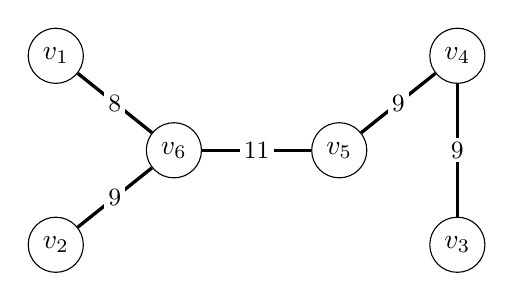
\begin{tikzpicture}[x=1.5cm,y=1.2cm,v/.style={circle,draw,inner sep=0pt,minimum size=7mm},w/.style={fill=white,inner sep=1.5pt,font=\small}]
\node[v] (1) at (0,1) {$v_1$};
\node[v] (6) at (1,0) {$v_6$};
\node[v] (2) at (0,-1) {$v_2$};
\node[v] (5) at (2.4,0) {$v_5$};
\node[v] (4) at (3.4,1) {$v_4$};
\node[v] (3) at (3.4,-1) {$v_3$};
\draw[very thick] (1)--node[w]{8}(6);
\draw[very thick] (2)--node[w]{9}(6);
\draw[very thick] (6)--node[w]{11}(5);
\draw[very thick] (5)--node[w]{9}(4);
\draw[very thick] (4)--node[w]{9}(3);
\end{tikzpicture}
\end{center}
\end{pastsoln}
